HTSLAM models the map as a hybrid topological-metric structure: the
environment is divided into a number of regions, and a local metric
map is built for each region. The relative poses of the regions are
stored in a topological structure. There is no global reference
frame. Only relative poses of the nearby regions are stored.

The motivation for the structure comes from a few sources. First,
dividing the world into a set of local maps appears to approximate the
way that humans reason \cite{psycho_kuipers82}. Second, is to ensure
that the mapping scheme scales to large environments.  The scalability
limitations of a single map SLAM methods are well known
\cite{guivant03,guivant01,guivant02} and prohibit real-time SLAM for
maps of practical size.  The third and final motivation is that a
robot does not require a single, global, metric description of the
world.  For example, in the ``fetch me a beer from the refrigerator''
task, there is no need for the robot to know the position of the
fridge while it is in the living room.  The robot only needs to know
the position of the fridge when it is near to the fridge.

This chapter describes the HTSLAM approach to map modelling.  Some
aspects of the map design are motivated by the mapping procedures
developed in chapter~\ref{chpt:Mapping} and so may only become fully
clear after reading chapter~\ref{chpt:Mapping}. The following section
describes the overall map structure.  Section~\ref{sec:local_map}
presents the methods used for modelling uncertainty within each local
map and section~\ref{sec:link} describes the methods used to model the
uncertainties of the topological links between maps.  Finally,
section~\ref{sec:region} discusses methods for defining the shape and
extent of each local region.

\section{Hybrid Map structure}
\label{sec:HM_structure}

\begin{figure}
\begin{center}
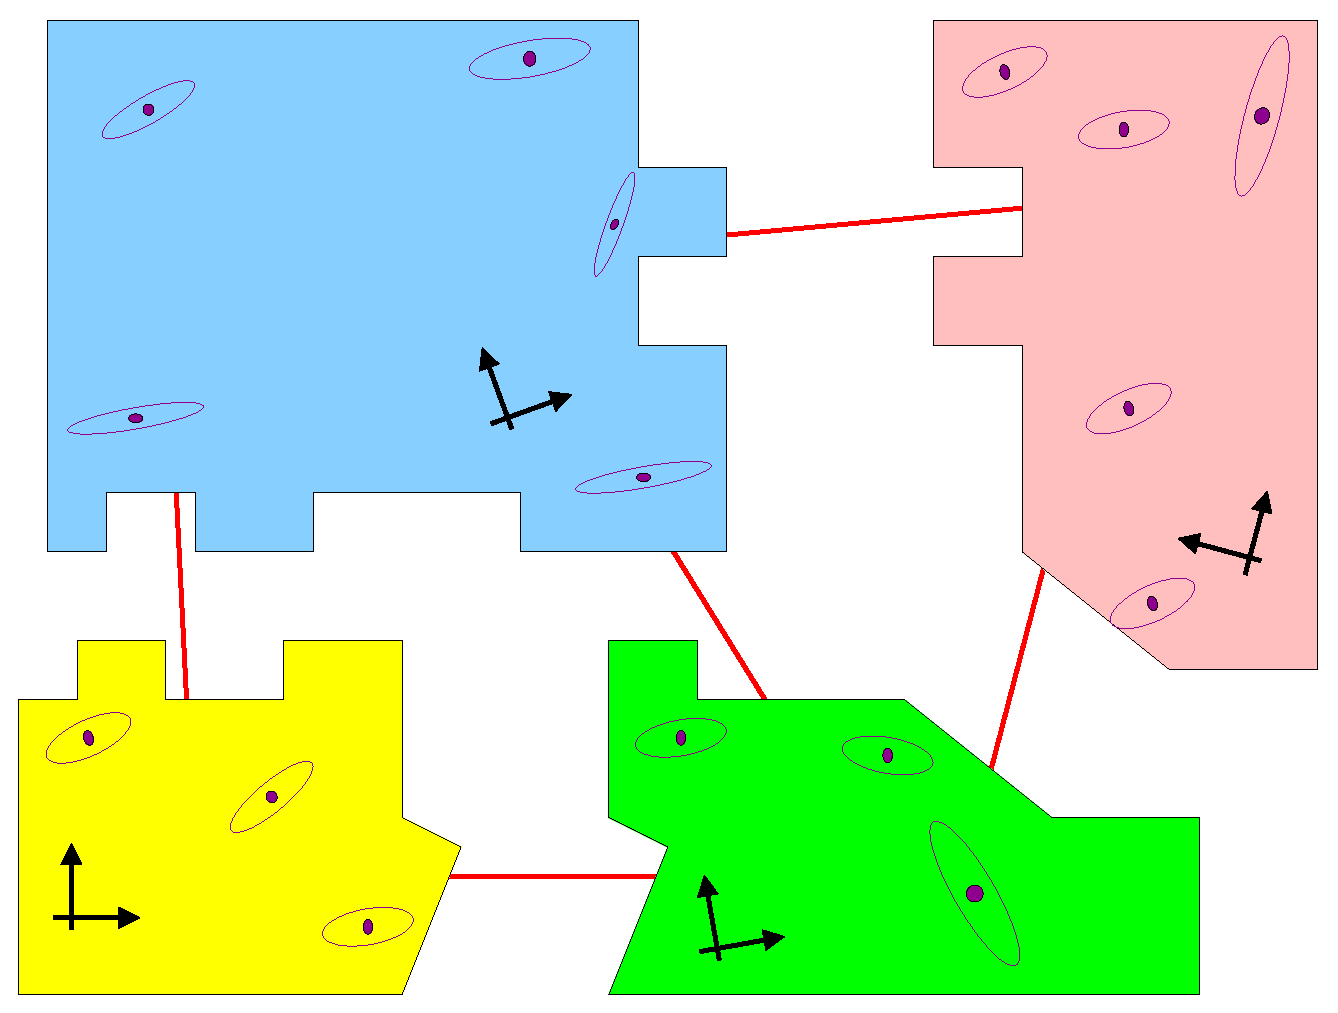
\includegraphics[width=10cm]{Pics/fig_map_structure}
\end{center}
\caption[Overview of HTSLAM map structure.]
{Overview of HTSLAM map structure. Each region has it's own
coordinate frame. The local map is built for every region (ellipses
erepresent landmarks). }
\label{fig:htslam_structure}
\end{figure}

\begin{figure}
\begin{center}
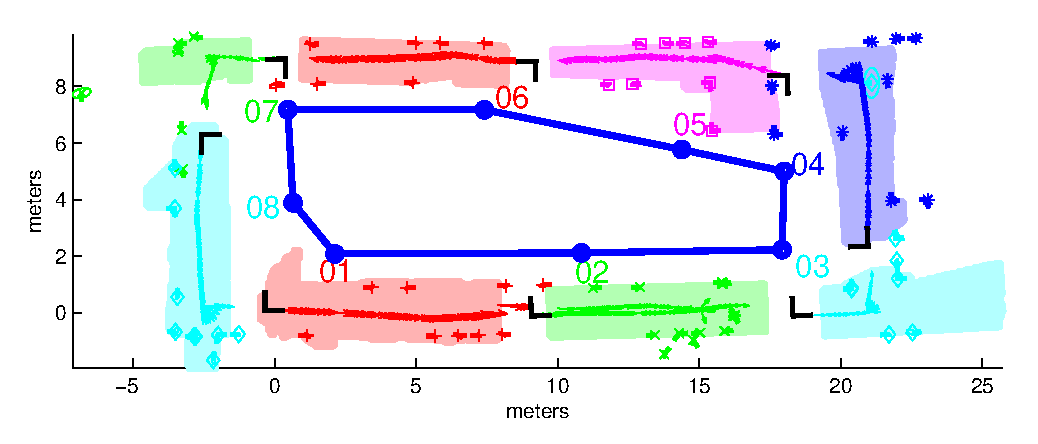
\includegraphics[width=14cm]{Pics/map_example_indoor}
\end{center}
\caption{Example of HTSLAM map for indoor environment}
\label{fig:htslam_structure_indoor}
\end{figure}


\begin{figure}
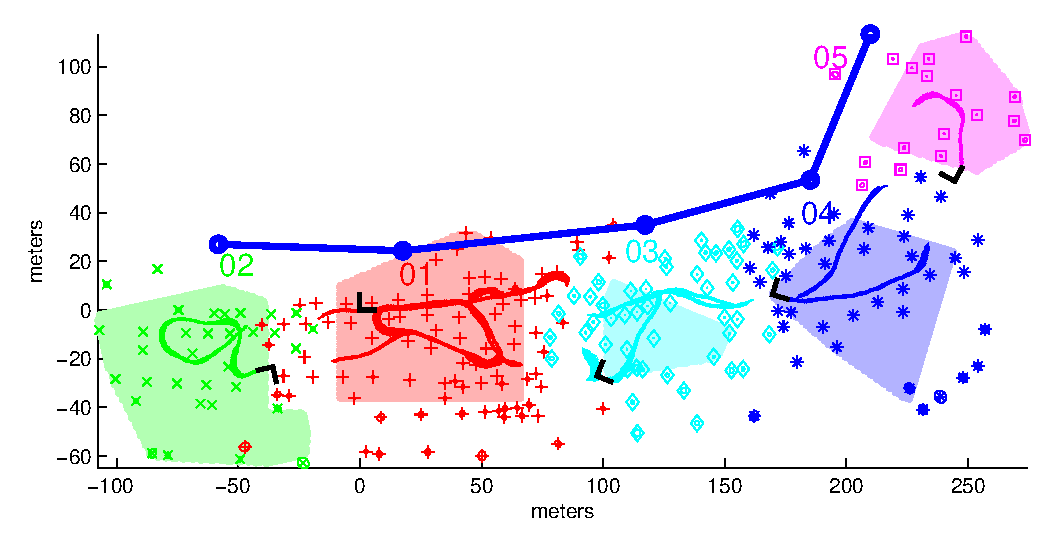
\includegraphics[width=14cm]{Pics/map_example_outdoor}
\caption{Example of HTSLAM map for outdoor environment}
\label{fig:htslam_structure_outdoor}
\end{figure}

In HTSLAM, a map is a connected graph. Every node of the graph
corresponds to a region within the environment. Each node has its own
reference frame and stores a local, metric map of the region and some
representation of the extent of the region in the local coordinate
frame. An example of HTSLAM map is given in the
\refFigure{fig:htslam_structure}. Note that there is no global reference
frame. The edges of the graph represent the stochastic coordinate
transformation between adjacent local maps
only. \refFigure{fig:htslam_structure_indoor} shows an example of an
HTSLAM map for indoor environment, and
\refFigure{fig:htslam_structure_outdoor} for an outdoor environment.

The structure used in HTSLAM is similar to that of \Atlas\ 
\cite{bosse02atlas}, however HTSLAM uses different uncertainty
representations, both for the coordinate transformations between
adjacent map frames and for the local maps. 
\Atlas as a framework allows to use arbitrary mapping model, however the two
implementations that have been published include EKF SLAM and scan matching.
\Atlas\ models the links or transitions between maps as Gaussian, and therefore
requires that the spatial uncertainty of the mapping module is represented as a Gaussian.
On the other hand, HTSLAM uses Rao-Blackwellised particle filter for the local maps (like FastSLAM), 
permitting multi-modal modelling of the local map. HTSLAM also models the transitions 
between maps using sets of particles.

A further difference between \Atlas\ and HTSLAM is that HTSLAM
maintains map extent information for every local map. This extra data
allows HTSLAM to perform map transitions and loop closing in a more
elegant way (as will be discussed later in
Chapter~\ref{chpt:LoopClosing}). In addition, HTSLAM explicitly
models the multiple hypotheses that arise during mapping, including
during loop closing, giving a more intuitively appealing and robust
approach.

The details of the uncertainty representation, both for each local map
and for the transitions between maps are discussed in the next two
sections.  Section~\ref{sec:region} discusses methods for
determining the extents of each local map.

\section{Modelling Uncertainty within a Local Map}
\label{sec:local_map}

To understand how uncertainty is represented within the local map, one
needs to be familiar with FastSLAM \cite{Montemerlo02d}, the mapping
scheme we use. An overview of FastSLAM was presented in
chapter~\ref{chpt:Overview}. In short, FastSLAM uses particles to
sample the possible paths of the robot. A map is built for each
path. Particles are evaluated based on how well the measurements match
the map.  Regular resampling is used to prune out unlikely paths.

The state $\s{k}{a}{m}$ of the $m$-th particle in the local map $a$
at time $k$ consists of the path of the particle within this local
frame, denoted \Xall{k}{a}{m}, and the map of the local environment
conditioned on the path, denoted \map{k}{a}{m}, i.e.
\begin{eqnarray}
 \s{k}{a}{m}    &=& [\Xall{k}{a}{m}, \map{k}{a}{m} ]\\
 \Xall{k}{a}{m} &=& [\x{0}{a}{m}, \x{1}{a}{m}, ... \x{k}{a}{m}]\\
 \map{k}{a}{m}  &=& [\mape{a}{m}{1}, \mape{a}{m}{2}, ..., \mape{a}{m}{n}],
\end{eqnarray}
where $\x{k}{a}{m}$ is the pose of a robot for the $m$-th particle at
time step $k$ in local map $a$ and $\mape{a}{m}{n}$ is the position of
an $n$-th landmark in local map $a$. The landmark position is a
stochastic variable, described by a Gaussian distribution. Note that
one does not have to store the whole path of a particle, since only
the most current pose of the particle is used in the mapping process.

A map is a probability distribution
$p(\map{k}{a}{m}|\Xall{k}{a}{m},\Zall{k}{a})$. If one makes an
assumptions that the map consists of landmarks, and that observations
are independent, then one can represent a map as a set of independent
landmarks, each conditioned on the path of a particle
$p(\mape{a}{m}{}|\Xall{k}{a}{m},\Zall{k}{a})$ (note that there is a
different map for each particle). FastSLAM approximates
$p(\mape{a}{m}{}|\Xall{k}{a}{m},\Zall{k}{a})$ with a Gaussian.  For
point landmarks, the distribution is a two-dimensional Gaussian
(location of the landmark on the plane). However, other landmark
characteristics can also be incorporated into the stochastic
variable. For example, if one builds a map of trees, the landmark
might have one extra parameter for the diameter of the tree trunk.
Note that since there are multiple particles, the actual posterior
distribution of the landmark is more complex than just a Gaussian. In
this thesis we will confine ourselves to planar motion. The results
however can be readily extended to full three-dimensional motion. Note
that, since the landmarks are estimated independently (in FastSLAM),
there is no need to maintain the global covariance matrix for the
whole map.

Each particle makes its own data association decisions. As a result,
the FastSLAM captures not only the uncertainty arising from the
continuous variables like robots' pose and the sensor measurements,
but also uncertainty due to discrete data association decisions.  This
uncertainty is not represented in the EKF approaches \cite{ekf_slam}.
The ability to capture this uncertainty is a big advantage, since in
most real-life situations the data association is ambiguous.

When mapping of a given local map is complete, the maps of all
particles alive at the time are stored within the local map. This set
of maps is effectively a sample from all the possible maps, given the
observations and odometry during the time robot was in the region.
Due to use of importance sampling, the sample from the maps is
expected to contain the most probable paths and their associated maps
(which are expected to be the better maps).

\section{Modelling Link Uncertainty}
\label{sec:link}
%Uncertainty of transformations

\begin{figure}
\begin{center}
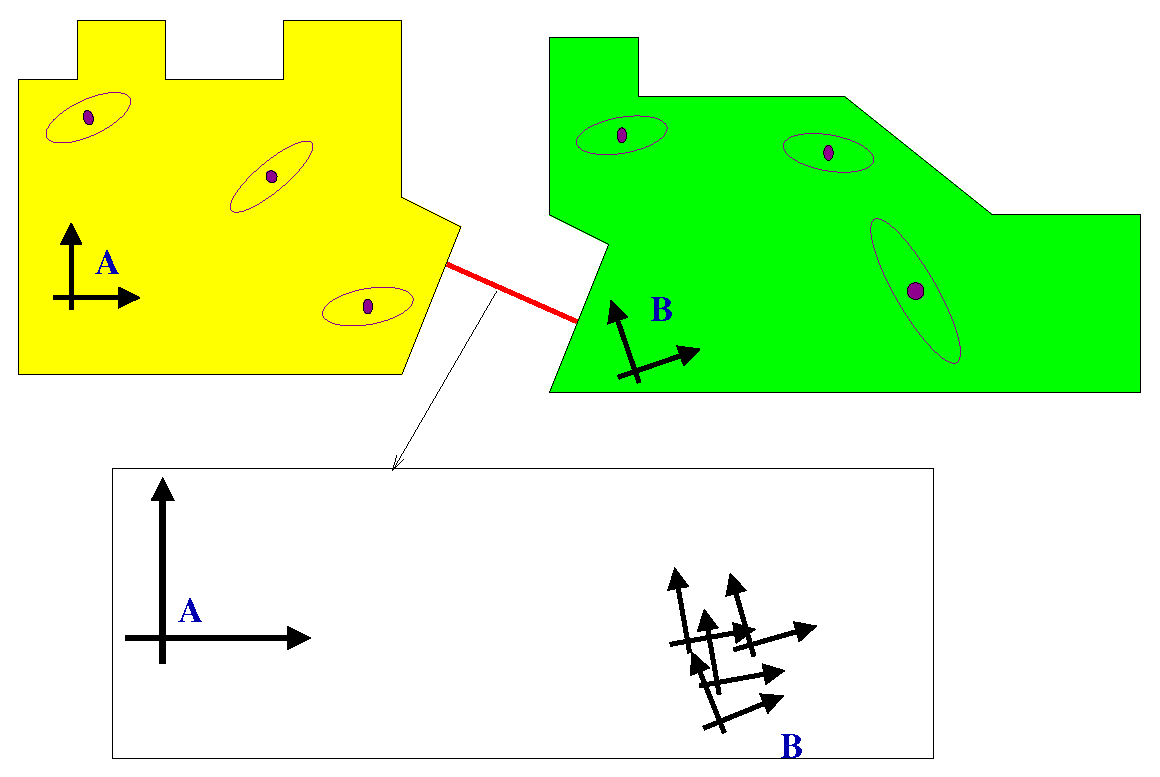
\includegraphics[width=10cm]{Pics/fig_transition_model}
\end{center}
\caption[Modeling transition distribution]
{Relative locations of the adjacent maps are represented by a
  set of particles.}
\end{figure}

The spatial relationships between adjacent local maps are each
represented by a set of particles.  As is common in SLAM
implementations, whenever a new map is started, the assumption is made
that the current location of the robot is precisely known in the new
map's coordinate frame.\footnote{Often it is assumed that the robot is
at the origin.  Here the position of the robot is chosen to place the
origin of the coordinate frame suitably for describing the local map
extents.} Thus, the transition between the old and the new map can be
most directly computed from the estimate of the robot pose in the old
map (a set of FastSLAM path particles) and the pose in the new map
(known by assumption). The transition is then a stochastic variable
which is most easily represented using particles. This is the chief
motivation for using a particle representation for the
transitions: the choice of representation makes the process of adding
new maps straightforward.

Note that when closing loops or, more generally, re-visiting maps,
there is no such easy method for transition determination and samples
must be taken from other distributions. For example, when closing
loops in HTSLAM, transition samples are taken from the results of map
matching (landmark matches are used to provide an estimate of
the transition function).

In general transitions and maps are not independent,
hence a joint probability needs to be stored. For adjacent maps $a$
and $b$ a joint probability distribution
$\prob{\map{}{}{a},\tr{}{a}{b}, \map{}{}{b}}$ is stored. Effectively,
the transition between the two adjacent maps captures a three-way
relationship between the two maps and the relative pose of the
reference frames of the two maps in a probabilistic manner. The exact
mechanism used to store the probability densities is described in more
detail in chapter~\ref{chpt:Mapping}.

It is worth noting that it is possible to derive the joint
probability $\prob{\map{}{}{a},\tr{}{a}{b},\map{}{}{b}}$ even for
non-adjacent maps $a$ and $b$ by merging probability densities along
the topological path joining the two maps.  The presence of loops in
the topological structure implies multiple paths between some of the
local maps. Therefore $\prob{\map{}{}{a},\tr{}{a}{b},\map{}{}{b}}$ can
be derived in several possible ways from the HTSLAM structure. This
adds a constraint to the HTSLAM structure, which will be discussed in
more detail in the chapter on loop closing(Chapter~\ref{chpt:LoopClosing}).

Let us define the coordinate transform using the \transit\ operator
\begin{equation}
\x{k}{}{b} = \x{k}{}{a} \transit \tr{}{a}{b}.
\end{equation}
This operator projects the pose of robot from one coordinate frame to
another.


\section{Defining Region Boundaries}
\label{sec:region}

Each region has its own ``area of influence''. This area is defined by
a grid map in the local reference frame. The size of the grid cells is
in the order of the robot's footprint, there is no need to have a
higher resolution. Regions who are neighbours in the topological
sense, have their region boundaries cropped in such a way as to
minimise the overlap. Since the grid maps are defined in local
coordinates, one needs to transform grids from one reference frame to
another, this is not a problem since relative poses of the
neighbouring maps are know with high certainty. The transformation is
therefore performed using the mean of the relative poses of the two
regions.


DELETE BELOW THE LINE\\
===============================

One of the important problems for HTSLAM is dividing the environment
into local maps. Ideally each local map should correspond to a unique
place in the environment. While the map structure used in HTSLAM is
self consistent even when the same region is mapped in two or more
different local maps, it is preferred to have a simpler representation
of the environment when possible.

There are two major reasons to split the environment into local
regions: to limit computational requirements and to reduce the effect
of the particle starvation problem.

Using regions addresses both of the problems outlined above. A finite
region implies a finite number of landmarks, from which follows bounds
on the computational requirements. Finite regions also imply limits on
the travelled distance, bounding the uncertainty of the robot pose,
hence banishing the effect of particle starvation within a region.

It seems natural for local maps to have non-overlapping areas. Having
unique regions also makes some of the mapping tasks significantly
easier. Deciding when to start a new map or when to switch to an
adjacent map frame becomes very straightforward when non-overlapping
regions are used. The regions are also used to initiate loop
closing. Having unique regions is potentially useful for human-robot
interaction, especially if regions correspond to human structures
like rooms or corridors.

It should be noted that non-overlapping constraints are only forced
locally. Only maps whose relative poses are known with high accuracy
are subject to this constraint. On a global scale maps can overlap
until a correspondence between the maps is proven by observation.

There are a number of factors to consider when choosing a particular
region modelling method:
\begin{itemize}
  \item \textbf{Environment:}
    
    Environment constraints the robot's motion and the sensor range.
    For example most robots are not capable of seeing or passing
    through walls. Region representations should capture these
    constraints in order to be useful.

  \item \textbf{Available sensors:}
    
    What information does a sensor provide? Is there a free-space sensor?
    What is the range of the mapping sensor? What is the angle of view
    of the mapping sensor? Typically, a region should not be smaller than
    the sensor range.
    
  \item \textbf{Exploration strategy:} 
    
    Is there feedback from the mapping module to the exploration
    module?  If the exploration module ensures that the whole region
    is explored before venturing into an unexplored region, then the
    region boundaries are independent of the robot's path. Otherwise
    the robot's path will have some impact on the local map region.

  \item \textbf{Computational constraints:}
    
    In situations when mapping is performed in real-time it is
    important to be able to compute the region quickly, and/or spread
    the computation over some time period, performing the task in the
    ``background'' between sensor readings.

\end{itemize}

\subsection{Operations on Local Map Regions}

HTSLAM requires the following operations to be supported by the
implementation of the region structure:

\begin{itemize}
\item It must be possible to determine the probability of a given
  point being inside the region. This probability can be either
  binary, a more general discrete function, or a continuous function
  of location.
 
\item A number of set operations should be supported:
  union, intersection and subtraction. Subtraction is used to
  determine non-overlapping maps. Map union is used in the situation
  when regions are joined (as might happen after loop closing).
  Finally, intersection is required for detecting overlap.

\end{itemize}

\subsection{Gaussian Ellipses}

Different region representations have been considered in this study.
Initially, elliptic regions using a two dimensional Gaussian was used.
The advantages of this representation include: easy computation,
straightforward implementation, low memory requirement. The disadvantages
are: no clear-cut boundaries between regions (i.e. can not force
non-overlapping), no straightforward strategy to re-evaluate regions
after closing the loop and lack of suitability for structured indoor
environments.

\subsection{Polygons}

Polygon representation of the map regions was also considered. The
idea is to fit a convex hull to the landmarks in the map. There are
two major problems with this approach. First, it is rather non-trivial
to enforce non-overlapping, especially when there are more than two
adjacent regions. Second, there might be a lot of ``free space'' left
between adjacent regions. This can then interfere with the mapping
algorithm, tricking the robot into starting a new map instead of
transferring into the neighbouring region.  In particular, it is
impossible to differentiate between the unexplored region and explored
but empty region with this approach.

\subsection{Grid-Based Model}

Finally, a grid map approach has been tried. The advantages of using
grid maps to store local map coverage information include:

\begin{itemize}
\item Set operations are clearly defined - easy to enforce
non-overlapping, while minimising the inter-region area.

\item Conceptually simple structure - easy to implement.

\item Works well in indoor environments.
\end{itemize}

On the negative side, a grid representation does require a lot more
memory than all other representations considered so far, however since
there is no need to a have a very fine detail, memory requirements are
kept low. For example a grid map with 10cm grid size will require 100
bytes per square meter. HTSLAM does not need access to all regions at
any one time, therefor the memory requirement is bounded.

\subsection{Defining the Local Map}

Possible techniques to initialise the local map region include:

\begin{itemize}
 \item Region snapshot from sensors at the very start.
 \item Incrementing region from sensors.
 \item Fixed initial size.
 \item Limiting the distance travelled by the robot, and then post-compute
 the region using landmarks and or robot path.
\end{itemize}

Most, if not all, autonomous robots require some form of free space
sensor on board to perform essential tasks of local path planning and
collision avoidance. This sensor can be used to compute an occupancy
grid of the region. The occupancy grid will then define the extent of
the local map. Computing an occupancy grid is a computationally
demanding task, but since high accuracy is not essential there is no
need to continually update it. Once the free space region has grown
``big enough'', the grid map is no longer updated.  Other
optimisations during computation of the occupancy grid might also
be possible.

Occupancy grids work well in the indoor environment, however for a
robot operating in the open space with just a few obstacles it is not
suitable. In such a situation a different approach for initialising
the mapping region should be used. One possibility is to assign a
fixed size polygon. This technique should work very well when the
exploration module is aware of the local map region and makes sure the
whole area is explored before leaving the region.

%Why is it a problem if the region is not completely explored? 
It is important that the local map does not claim a chunk of space
that wasn't actually explored. A robot needs to be able to localise
well within a local map when it enters the area claimed by the map. In
order to achieve this, the probability that the robot observes at
least some landmarks when entering the region should be maximised. It
is best to add new landmarks to the map while still observing some of
the existing landmarks, that keeps the quality of the map higher (it
relates to the particles deprivation problem, we have only so many
particles to work with, this has to be explained better, but maybe not
here. Reference to chapter on map building procedure)

In a situation where the mapping module has no influence on where the
robot goes, additional complications occur. Since it is impossible to
predict or influence the robots path in any way, the mapping module
has to either delay computation of the region or make some assumptions
about the future path of the robot.

One approach is to assign a fixed size chunk of space to the local
map, and hope that it will be mapped well enough, regardless of the
path the robot will take. Another possibility is to trim down the
region after mapping is complete. There are several ways to accomplish
this. The main problem with this approach is that the robot might
leave the area very quickly, so the region might be trimmed to almost
nothing. In such situation some non-trivial region merging should
occur.

\SILENT{
Several approaches can be used to trim down the region. It is possible
to use the map that was built. For example, find a convex hull of the
map (use only good enough i.e. certain landmarks). Use intersection of
the convex hull with the initial area as the new region area. That is
the approach used to process the Victoria park data set, and it works
quite well.  

Or maybe an easier solution - fit a Gaussian to the map,
and then use intersection of the 3( or 4, or 5) sigma ellipse with the
initial grid. Another way is to use robots path only. Assume a certain
coverage area for the robots pose (in robot centred coordinates, for
example a square, or a sensor range sector), then compute an
intersection of the robots path with the initial region grid map,
using this coverage area. This can be computed incrementally as the
robot explores the regions, hence it is more real-time friendly. This
is essentially equivalent to a free space approach, except that
instead of ``probably free'' space we use ``probably was observed''
space.
}

% LocalWords:  HTSLAM FastSLAM resampling EKF odometry
